\documentclass[a4paper]{article}

\def\npart {SUROP}
\def\nterm {Summer 2016}
\def\ncourse {Shadow tomography}

% Imports

\usepackage[pdftex,colorlinks=true]{hyperref}
\usepackage[T1]{fontenc}
\usepackage{lipsum}
\usepackage{amsfonts}
\usepackage{amsmath}
\usepackage{amssymb}
\usepackage{amsthm}
\usepackage{booktabs}
\usepackage{caption}
\usepackage{enumitem}
\usepackage{graphicx}
\usepackage{mathtools}
\usepackage{microtype}
\usepackage{multirow}
\usepackage{pdfpages}
\usepackage{siunitx}
\usepackage{tabularx}
\usepackage{tikz}
\usepackage{todo}
\usepackage{fancyhdr}
\usepackage{ifthen}
\usepackage[normalem]{ulem}
\usepackage{pdflscape}
\usepackage{lmodern}
\usepackage{listings}
\usepackage{floatrow}%

\pagestyle{fancyplain}
\lhead{\emph{\nouppercase{\leftmark}}}
\ifx \nextra \undefined 
  \rhead{\ifthenelse{\value{page}=1}{}{\npart\ \ncourse}}
\else
  \rhead{\ifthenelse{\value{page}=1}{}{\npart\ \ncourse\ (\nextra)}}
\fi
\usetikzlibrary{arrows}
\usetikzlibrary{decorations.markings}
\usetikzlibrary{positioning}
\usetikzlibrary{calc}

% Theorems
\theoremstyle{definition}
\newtheorem*{aim}{Aim}
\newtheorem*{axiom}{Axiom}
\newtheorem*{claim}{Claim}
\newtheorem*{cor}{Corollary}
\newtheorem*{defi}{Definition}
\newtheorem*{eg}{Example}
\newtheorem*{fact}{Fact}
\newtheorem*{law}{Law}
\newtheorem*{lemma}{Lemma}
\newtheorem*{notation}{Notation}
\newtheorem*{prop}{Proposition}
\newtheorem*{thm}{Theorem}

% Latex constructs
\newcommand{\mb}[1]{\mathbf{#1}}
\newcommand{\note}{\vspace{3pt}\noindent \emph{Note}:\;}
\newcommand{\argmin}{\operatornamewithlimits{argmin}}

\renewcommand{\labelitemi}{--}
\renewcommand{\labelitemii}{$\circ$}
\renewcommand{\labelenumi}{(\roman{*})}

\let\stdpart\part
\renewcommand\part{\newpage\stdpart}

\let\stdsection\section
\renewcommand\section{\stdsection}

\newcommand{\img}[2][]{\begin{center}\centering\includegraphics[#1]{images/#2.pdf}\end{center}}

% Strike through
\def\st{\bgroup \ULdepth=-.55ex \ULset}

% Maths symbols
\newcommand{\bra}{\langle}
\newcommand{\ket}{\rangle}

\newcommand{\N}{\mathbb{N}}
\newcommand{\Z}{\mathbb{Z}}
\newcommand{\Q}{\mathbb{Q}}
\newcommand{\R}{\mathbb{R}}
\newcommand{\C}{\mathbb{C}}
\newcommand{\Prob}{\mathbb{P}}
\renewcommand{\P}{\mathbb{P}}
\newcommand{\E}{\mathbb{E}}
\newcommand{\F}{\mathbb{F}}
\newcommand{\cU}{\mathcal{U}}

\DeclareMathOperator{\im}{Im}
\DeclareMathOperator{\re}{Re}

\DeclareMathOperator{\tr}{tr}
\DeclareMathOperator{\diag}{diag}
\DeclareMathOperator{\rank}{rank}
\DeclareMathOperator{\card}{card}
\DeclareMathOperator{\spn}{span}

\DeclareMathOperator{\erf}{erf}
\DeclareMathOperator{\erfc}{erfc}

\DeclareMathOperator{\ord}{ord}
\DeclareMathOperator{\Sym}{Sym}

\DeclareMathOperator{\sgn}{sgn}
\DeclareMathOperator{\orb}{orb}
\DeclareMathOperator{\stab}{stab}
\DeclareMathOperator{\ccl}{ccl}

\DeclareMathOperator{\lcm}{lcm}
\DeclareMathOperator{\hcf}{hcf}

\DeclareMathOperator{\Int}{Int}
\DeclareMathOperator{\id}{id}

\DeclareMathOperator{\betaD}{beta}
\DeclareMathOperator{\gammaD}{gamma}
\DeclareMathOperator{\Poisson}{Poisson}
\DeclareMathOperator{\binomial}{binomial}
\DeclareMathOperator{\multinomial}{multinomial}
\DeclareMathOperator{\Bernoulli}{Bernoulli}
\DeclareMathOperator{\like}{like}

\DeclareMathOperator{\var}{var}
\DeclareMathOperator{\cov}{cov}
\DeclareMathOperator{\bias}{bias}
\DeclareMathOperator{\mse}{mse}
\DeclareMathOperator{\corr}{corr}

\DeclareMathOperator{\otp}{otp}
\DeclareMathOperator{\dom}{dom}

\newcommand{\GL}{\mathrm{GL}}
\newcommand{\SL}{\mathrm{SL}}
\newcommand{\Or}{\mathrm{O}}
\newcommand{\SO}{\mathrm{SO}}
\newcommand{\U}{\mathrm{U}}
\newcommand{\SU}{\mathrm{SU}}

\renewcommand{\d}{\mathrm{d}}

\tikzset{->/.style = {decoration={markings,
                                  mark=at position 1 with {\arrow[scale=2]{latex'}}},
                      postaction={decorate}}}
\tikzset{<-/.style = {decoration={markings,
                                  mark=at position 0 with {\arrowreversed[scale=2]{latex'}}},
                      postaction={decorate}}}
\tikzset{<->/.style = {decoration={markings,
                                   mark=at position 0 with {\arrowreversed[scale=2]{latex'}},
                                   mark=at position 1 with {\arrow[scale=2]{latex'}}},
                       postaction={decorate}}}
\tikzset{->-/.style = {decoration={markings,
                                   mark=at position #1 with {\arrow[scale=2]{latex'}}},
                       postaction={decorate}}}
\tikzset{-<-/.style = {decoration={markings,
                                   mark=at position #1 with {\arrowreversed[scale=2]{latex'}}},
                       postaction={decorate}}}

\tikzset{circ/.style = {fill, circle, inner sep = 0, minimum size = 3}}


\begin{document}
\title{
    SUROP \\ Progress report
}
\title{Summer Undergraduate Research Opportunities}
\date{July, 2016}
\author{Emile Okada \\ University of Cambridge}
\maketitle

\newpage

\setcounter{section}{0}
\section{Week 1}
\subsection{Reading}
I started the week reading Chapter 1 section 2 of Charles L. Epstein's "Introduction to the Mathematics of Medical Imaging".
It covered how to reconstuct a 2D convex object from the shadows of an object. 
If $h(\theta)$ is the shadow function as described in the book (essentially the distance of the support line in direction $(-\sin(\theta),\cos(\theta))$ from the origin), then the convex hull can be parameterized by

\begin{equation}
    (x(\theta),y(\theta)) = h(\theta)\cdot(\cos(\theta),\sin(\theta))+h'(\theta)\cdot(-\sin(\theta),\cos(\theta)).
\end{equation}

We can extend this idea to 3D by considering slices of the object. 
Fix some vector {\bfseries v} and then consider the collection of planes perpendicular to {\bfseries v}. 
In each of the planes one can use the 2D method to construct a 2D convex hull of the intersection of the object with the plane. 
Stringing all these 2D slices together then gives a rough reconstruction of the 3D object from its shadows.

I also spent some time reading up on the TV transform and scale spaces, to get a rough idea of which project I'd like to do. 
I ended up going with the tomography project, but spend roughly 1.5 days doing reading for the other project.

\subsubsection{Remaining tasks}
The above method only allows for 'slicewise convex' reconstructions. While better than convex, this doesn't ustilize all the data available from the shadows e.g. see the rabit ears below. We know the two ears are two separate 'blobs' and we can tell this from the shadow, but this information is nonetheless lost in the reconstruction. I will try to find ways on how to improve on this (so that e.g. if we scan a human we can see two legs rather than one large blob).

\subsection{Coding}
On Thursday I started coding. 
To have some examples to work with I used the Wolfram Mathematica ExampleData function to obtain a 3D model of a rabit.

\begin{figure}[H]
  \centering
    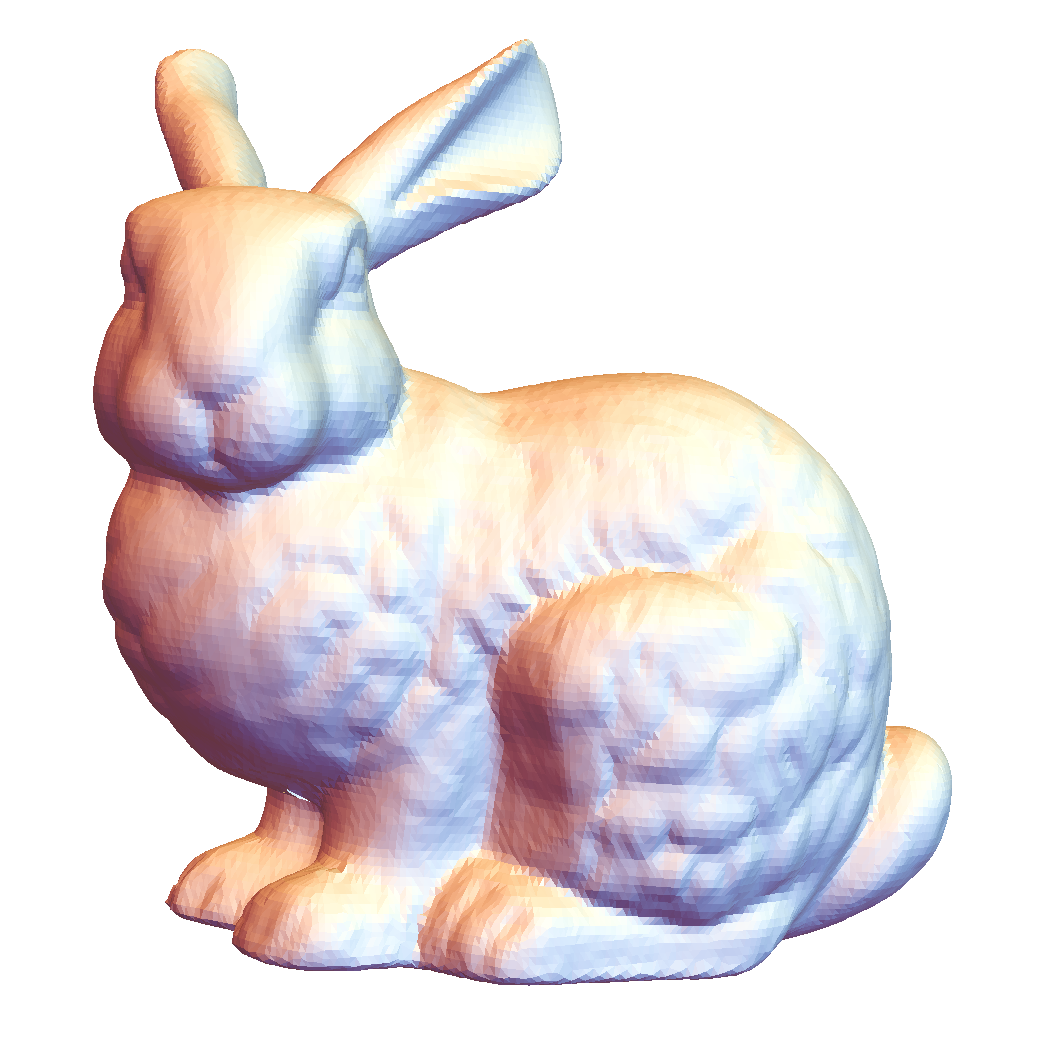
\includegraphics[width=0.4\textwidth]{figures/3D_rabit.png}
    \caption{3D model of a rabit from Mathematica ExampleData.}
  \label{fig:f2}
\end{figure}

I then took its orthogonal projection and binarized the image to obtain shadows of the rabit from 10 different angles.

\begin{figure}[H]
    \begin{floatrow}
        \ffigbox{
\includegraphics[scale = 0.5]{figures/space1.jpg}}{\caption{Shadow of rabit with $\theta=0$}\label{fig:err1}}
        \ffigbox{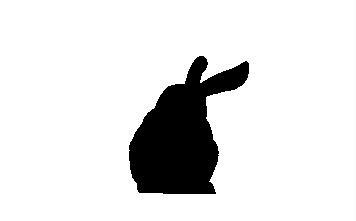
\includegraphics[scale = 0.5]{figures/space5.jpg}}{\caption{Shadow of rabit with $\theta=\pi/2$}\label{fig:err2}}
    \end{floatrow}
\end{figure}

I then finished writing the code for reconstructing the object from its shadows in python (see page \pageref{alg:shadow} or my \href{https://github.com/emileokada/image3d}{github}) on Friday.

\begin{figure}[H]
  \centering
    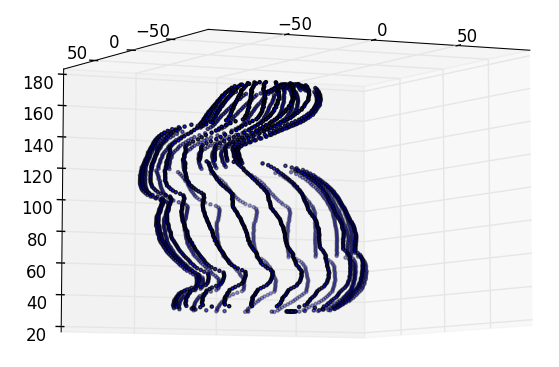
\includegraphics[width=0.7\textwidth]{figures/rabit.png}
    \caption{Reconstruction of the rabit using the script on page \pageref{alg:shadow}.}
  \label{fig:f2}
\end{figure}

\subsubsection{Challenges}
I had some problems originally with taking the derivative of the shadow function since the input was a bit noisy.
To fix this problem I convolved the data with a discrete gaussian (binomial distribution) to smooth out the noise.
This worked well with the example data. 
However, it remains to see whether it will work well enough for the actual real life pictures which will probably be a lot more noisy.

\subsubsection{Remaining tasks}
There are currently a lot more data points than I need. At the moment I'm calculating the shadow function fow each row of the image matrix.
This results in a lot of points which causes the rendering to take some time.
I can probably get away with a lot fewer points in the z direction.
I also plan on adding a polygonal mesh so it looks a bit nicer.
Lastly, I should probably also do some smoothing in the z direction to fix the sudden cutoffs that tend to occur when the variations in the 3D object are smaller than the 'resolution' in the z-direction.

\begin{figure}[H]
  \centering
    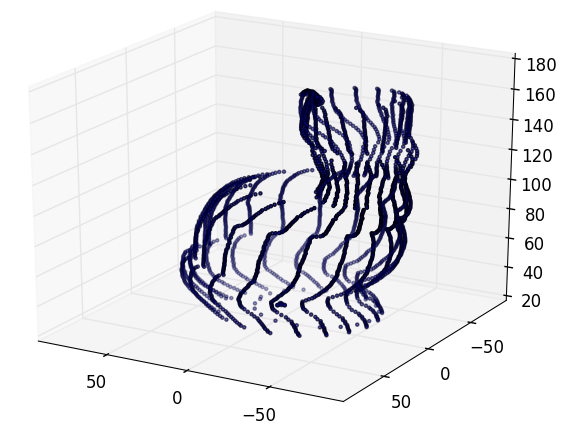
\includegraphics[width=0.7\textwidth]{figures/ear_and_back_cutoff.png}
    \caption{Cutoff of rabits ears. Can probably be fixed by smoothing the data in the z direction.}
  \label{fig:f2}
\end{figure}

\subsection{Building}
I haven't begun building yet, but I now have a rough idea of the the set should look like. 
At the moment I'm thinking of creating a simple turn table (rotating platform) on which a person stands. I'll then place some bright lights in front for them and a big white sheet of paper behind on which to shine their shadow. 
A camera is then placed behind the paper to capture the shadows.

\subsubsection{Remaining tasks}
I'll create a proper design this week and make a basic prototype on a smaller scale hopefully by next week.

\newpage
\section{Code}
\subsection{3D reconstruction from shadows}
\label{alg:shadow}
\lstinputlisting[language=Python]{../shadow_function.py}
\subsection{Miscellaneous functions}
\label{alg:misc}
\lstinputlisting[language=Python]{../misc.py}
\end{document}

